%%%%%%%%%%%%%%%%%%%%%%%%%%%%%%%%%%%%%%%%%
% Programming/Coding Assignment
% LaTeX Template
%
% This template has been downloaded from:
% http://www.latextemplates.com
%
% Original author:
% Ted Pavlic (http://www.tedpavlic.com)
%
% Note:
% The \lipsum[#] commands throughout this template generate dummy text
% to fill the template out. These commands should all be removed when 
% writing assignment content.
%
% This template uses a Perl script as an example snippet of code, most other
% languages are also usable. Configure them in the "CODE INCLUSION 
% CONFIGURATION" section.
%
%%%%%%%%%%%%%%%%%%%%%%%%%%%%%%%%%%%%%%%%%

%----------------------------------------------------------------------------------------
%	PACKAGES AND OTHER DOCUMENT CONFIGURATIONS
%----------------------------------------------------------------------------------------

\documentclass{article}

\usepackage{fancyhdr} % Required for custom headers
\usepackage{lastpage} % Required to determine the last page for the footer
\usepackage{extramarks} % Required for headers and footers
\usepackage[usenames,dvipsnames]{color} % Required for custom colors
\usepackage{graphicx} % Required to insert images
\usepackage{subcaption}
\usepackage{listings} % Required for insertion of code
\usepackage{courier} % Required for the courier font
\usepackage{lipsum} % Used for inserting dummy 'Lorem ipsum' text into the template
\usepackage{amsfonts}
\usepackage{amssymb}
\usepackage{amsmath}
\usepackage{enumerate}
\usepackage{soul}
%Code for including Python code in Latex - outlined on the Piazza forum post, taken from Stackoverflow

\usepackage{enumitem}
\usepackage[utf8]{inputenc}
\definecolor{dkgreen}{rgb}{0,0.6,0}
\definecolor{gray}{rgb}{0.5,0.5,0.5}
\definecolor{mauve}{rgb}{0.58,0,0.82}

\lstset{frame=tb,
  language=Python,
  aboveskip=3mm,
  belowskip=3mm,
  showstringspaces=false,
  columns=flexible,
  basicstyle={\small\ttfamily},
  numbers=none,
  numberstyle=\tiny\color{gray},
  keywordstyle=\color{blue},
  commentstyle=\color{dkgreen},
  stringstyle=true{mauve},
  breaklines=true,
  breakatwhitespace=true,
  tabsize=3
}

% Margins
\topmargin=-0.45in
\evensidemargin=0in
\oddsidemargin=0in
\textwidth=6.5in
\textheight=9.0in
\headsep=0.25in

% Paragraph spacing
\setlength{\parskip}{10pt}


\linespread{1.1} % Line spacing

% Set up the header and footer
\pagestyle{fancy}
\lhead{\hmwkAuthorName} % Top left header
\chead{\hmwkClass\ (\hmwkClassTime): \hmwkTitle} % Top center head
%\rhead{\firstxmark} % Top right header
\lfoot{\lastxmark} % Bottom left footer
\cfoot{} % Bottom center footer
\rfoot{Page\ \thepage\ of\ \protect\pageref{LastPage}} % Bottom right footer

\setlength\parindent{0pt} % Removes all indentation from paragraphs

%----------------------------------------------------------------------------------------
%	CODE INCLUSION CONFIGURATION
%----------------------------------------------------------------------------------------

\definecolor{MyDarkGreen}{rgb}{0.0,0.4,0.0} % This is the color used for comments
\lstloadlanguages{Perl} % Load Perl syntax for listings, for a list of other languages supported see: ftp://ftp.tex.ac.uk/tex-archive/macros/latex/contrib/listings/listings.pdf
\lstset{language=Perl, % Use Perl in this example
        frame=single, % Single frame around code
        basicstyle=\small\ttfamily, % Use small true type font
        keywordstyle=[1]\color{Blue}\bf, % Perl functions bold and blue
        keywordstyle=[2]\color{Purple}, % Perl function arguments purple
        keywordstyle=[3]\color{Blue}\underbar, % Custom functions underlined and blue
        identifierstyle=, % Nothing special about identifiers                                         
        commentstyle=\usefont{T1}{pcr}{m}{sl}\color{MyDarkGreen}\small, % Comments small dark green courier font
        stringstyle=\color{Purple}, % Strings are purple
        showstringspaces=false, % Don't put marks in string spaces
        tabsize=5, % 5 spaces per tab
        %
        % Put standard Perl functions not included in the default language here
        morekeywords={rand},
        %
        % Put Perl function parameters here
        morekeywords=[2]{on, off, interp},
        %
        % Put user defined functions here
        morekeywords=[3]{test},
       	%
        morecomment=[l][\color{Blue}]{...}, % Line continuation (...) like blue comment
        numbers=left, % Line numbers on left
        firstnumber=1, % Line numbers start with line 1
        numberstyle=\tiny\color{Blue}, % Line numbers are blue and small
        stepnumber=5 % Line numbers go in steps of 5
}

% Creates a new command to include a perl script, the first parameter is the filename of the script (without .pl), the second parameter is the caption
\newcommand{\perlscript}[2]{
\begin{itemize}
\item[]\lstinputlisting[caption=#2,label=#1]{#1.pl}
\end{itemize}
}

%----------------------------------------------------------------------------------------
%	DOCUMENT STRUCTURE COMMANDS
%	Skip this unless you know what you're doing
%----------------------------------------------------------------------------------------

% Header and footer for when a page split occurs within a problem environment
\newcommand{\enterProblemHeader}[1]{
%\nobreak\extramarks{#1}{#1 continued on next page\ldots}\nobreak
%\nobreak\extramarks{#1 (continued)}{#1 continued on next page\ldots}\nobreak
}

% Header and footer for when a page split occurs between problem environments
\newcommand{\exitProblemHeader}[1]{
%\nobreak\extramarks{#1 (continued)}{#1 continued on next page\ldots}\nobreak
%\nobreak\extramarks{#1}{}\nobreak
}

\setcounter{secnumdepth}{0} % Removes default section numbers
\newcounter{homeworkProblemCounter} % Creates a counter to keep track of the number of problems
\setcounter{homeworkProblemCounter}{-1}

\newcommand{\homeworkProblemName}{}
\newenvironment{homeworkProblem}[1][Problem \arabic{homeworkProblemCounter}]{ % Makes a new environment called homeworkProblem which takes 1 argument (custom name) but the default is "Problem #"
\stepcounter{homeworkProblemCounter} % Increase counter for number of problems
\renewcommand{\homeworkProblemName}{#1} % Assign \homeworkProblemName the name of the problem
\section{\homeworkProblemName} % Make a section in the document with the custom problem count
\enterProblemHeader{\homeworkProblemName} % Header and footer within the environment
}{
\exitProblemHeader{\homeworkProblemName} % Header and footer after the environment
}

\newcommand{\problemAnswer}[1]{ % Defines the problem answer command with the content as the only argument
\noindent\framebox[\columnwidth][c]{\begin{minipage}{0.98\columnwidth}#1\end{minipage}} % Makes the box around the problem answer and puts the content inside
}

\newcommand{\homeworkSectionName}{}
\newenvironment{homeworkSection}[1]{ % New environment for sections within homework problems, takes 1 argument - the name of the section
\renewcommand{\homeworkSectionName}{#1} % Assign \homeworkSectionName to the name of the section from the environment argument
\subsection{\homeworkSectionName} % Make a subsection with the custom name of the subsection
\enterProblemHeader{\homeworkProblemName\ [\homeworkSectionName]} % Header and footer within the environment
}{
\enterProblemHeader{\homeworkProblemName} % Header and footer after the environment
}

%----------------------------------------------------------------------------------------
%	NAME AND CLASS SECTION
%----------------------------------------------------------------------------------------

\newcommand{\hmwkTitle}{Assignment 1} % Assignment title
\newcommand{\hmwkDueDate}{Friday,\ February 23,\ 2018} % Due date
\newcommand{\hmwkClass}{CSC2515} % Course/class
\newcommand{\hmwkClassTime}{L0101} % Class/lecture time
\newcommand{\hmwkAuthorName}{Matthew Wong, Susanne Pyda} % Your name

%----------------------------------------------------------------------------------------
%	TITLE PAGE
%----------------------------------------------------------------------------------------

\title{
\vspace{2in}
\textmd{\textbf{\hmwkClass:\ \hmwkTitle}}\\
\normalsize\vspace{0.1in}\small{Due\ on\ \hmwkDueDate}\\
\vspace{0.1in}
\vspace{3in}
}

\author{\textbf{\hmwkAuthorName}}
%\date{} % Insert date here if you want it to appear below your name

%----------------------------------------------------------------------------------------

\begin{document}

\maketitle
\clearpage
%----------------------------------------------------------------------------------------
%	Introduction
%----------------------------------------------------------------------------------------

\begin{homeworkProblem}

\noindent \textit{Introductory information and readme instructions}

Attached, you will find the required submissions \textit{digits.py, faces.py, deepfaces.py, deepnn.tex  \& faces.pdf} in addition to two folders - both containing an appropriate amount of pictures for each actor/actress.  Comments about the code are located in each of the source files. Code was written in Python 3.5 with the Anaconda environment - the packages used are outlined at the beginning of the file.



\end{homeworkProblem}
\clearpage
%----------------------------------------------------------------------------------------
%	PROBLEM 1
%----------------------------------------------------------------------------------------

% To have just one problem per page, simply put a \clearpage after each problem

\begin{homeworkProblem}

\noindent \textit{Dataset description}

TALK ABOUT MNIST DATASET HERE - make some BS up, who cares

\end{homeworkProblem}
\clearpage
%----------------------------------------------------------------------------------------
%	PROBLEM 2
%----------------------------------------------------------------------------------------

\begin{homeworkProblem}
\noindent \textit{Computation of the provided Network.}

The source code to compute the assigned network is provided below.
\begin{lstlisting}
def compute(X, W, b):
    hypothesis = np.matmul(W.T, X)
    hypothesis = hypothesis + b
    return hypothesis
\end{lstlisting}

The source code running a test case of the assigned network is provided below, followed by the output.  M is the MNIST dataset provided, W and b are randomly initialized numpy variables.
\begin{lstlisting}
def testPart2():
    # Load Data
    M = loadData()
    train = loadTrain(M)
    # Testing computation function
    # Initialize weights and bias to random normal variables
    W = np.random.normal(0.0, 0.1, (784, 10))
    b = np.random.normal(0, 0.1, (10, 1))
    hypothesis = compute(train, W, b)
    print(softmax(hypothesis))
\end{lstlisting}

Output from the test case:
\begin{lstlisting}
[[ 0.02681158  0.0532326   0.04155301 ...,  0.02401518  0.05461363
   0.09298066]
 [ 0.02934882  0.02945978  0.00866719 ...,  0.02812303  0.05160524
   0.06640991]
 [ 0.07800929  0.14095711  0.05324094 ...,  0.08344358  0.071218
   0.03403779]
 ..., 
 [ 0.06811845  0.09068319  0.11408343 ...,  0.09293973  0.23242635
   0.24750088]
 [ 0.42558937  0.28527524  0.36294473 ...,  0.32821263  0.12923604
   0.11150445]
 [ 0.04023265  0.03443131  0.05201543 ...,  0.0454216   0.06806685
   0.08509415]]
\end{lstlisting}
\end{homeworkProblem}
\clearpage
%----------------------------------------------------------------------------------------

%----------------------------------------------------------------------------------------
%	PROBLEM 3
%----------------------------------------------------------------------------------------

\begin{homeworkProblem}
\noindent \textit{Gradient derivation and vectorized format}

\begin{enumerate}[label=(\Alph*)]
\item NEED TO WRITE THE PROOF HERE
\item The source code for computing the gradient is shown below.
\begin{lstlisting}
def grad_NLL_W(y, o, layer):
    p = softmax(o)
    grad = p - y
    grad = np.matmul(grad, np.transpose(layer))
    return np.transpose(grad)


# Computes the gradient of negative log-loss function for biases only
def grad_NLL_b(y, o):
    p = softmax(o)
    grad = p - y
    grad = np.sum(grad, axis=1, keepdims=True)
    return grad
\end{lstlisting}
The source for our test cases, along with the outputs, are also shown below.
\begin{lstlisting}
def testPart3():
    # Test gradient functionality
    y = np.zeros((10, 1))
    y[1, :] = 1

    # Create a test matrix
    M = loadData()
    test0 = ((M["train1"][130].T) / 255.0).reshape((784, 1))
    W = np.random.normal(0, 0.2, (784, 10))
    b = np.random.normal(0, 0.2, (10, 1))
    # print(np.where(test0 != 0))

    # Create a finite difference
    h = 0.00001

    # Weight testing
    finite_W = np.zeros((784, 10))
    finite_W[542, 0] = h
    finite_d = (NLL(y, compute(test0, W + finite_W, b)) - NLL(y, compute(test0, W, b))) / (h)
    print("Cost for row 542, column 0: " + str(finite_d))
    gradient = grad_NLL_W(y, compute(test0, W, b), test0)
    print("Gradient for row 542, column 0: " + str(gradient[542, 0]))

    # Bias testing
    finite_b = np.zeros((10, 1))
    finite_b[1, :] = h
    finite_d = (NLL(y, compute(test0, W, b + finite_b)) - NLL(y, compute(test0, W, b))) / (h)
    print("Cost for second element in bias: " + str(finite_d))
    gradient = grad_NLL_b(y, compute(test0, W, b))
    print("Gradient matrix: " + str(gradient))

    # Reinitialize test variables for another test
    finite_W = np.zeros((784, 10))
    finite_b = np.zeros((10, 1))
    y = np.zeros((10, 1))
    test1 = ((M["train9"][130].T) / 255.0).reshape((784, 1))
    y[9, :] = 1

    # Weight testing
    finite_W[300, 4] = h
    finite_d = (NLL(y, compute(test1, W + finite_W, b)) - NLL(y, compute(test1, W, b))) / (h)
    print("Cost for row 300, column 4: " + str(finite_d))
    gradient = grad_NLL_W(y, compute(test1, W, b), test1)
    print("Gradient for row 300, column 4: " + str(gradient[300, 4]))

    # Bias testing
    finite_b[4, :] = h
    finite_d = (NLL(y, compute(test1, W, b + finite_b)) - NLL(y, compute(test1, W, b))) / (h)
    print("Cost for fifth element in bias: " + str(finite_d))
    gradient = grad_NLL_b(y, compute(test1, W, b))
    print("Gradient matrix: " + str(gradient))

\end{lstlisting}
\begin{lstlisting}
Cost for row 542, column 0: 0.0424078520744
Gradient for row 542, column 0: 0.0424076964593
Cost for second element in bias: -0.996437311773
Gradient matrix: [[ 0.05461597]
 [-0.99643733]
 [ 0.03592502]
 [ 0.32774037]
 [ 0.04444944]
 [ 0.05179153]
 [ 0.08930539]
 [ 0.14572631]
 [ 0.19441422]
 [ 0.05246907]]
Cost for row 300, column 4: 0.000106382902487
Gradient for row 300, column 4: 0.000106382357955
Cost for fifth element in bias: 0.00010680176743
Gradient matrix: [[  3.36017608e-03]
 [  1.57850465e-02]
 [  1.07051677e-02]
 [  1.06504072e-01]
 [  1.06801186e-04]
 [  6.75277789e-02]
 [  9.15366897e-02]
 [  8.16717644e-02]
 [  6.16811862e-01]
 [ -9.94009358e-01]]
\end{lstlisting}
\end{enumerate}


\end{homeworkProblem}
\clearpage
%----------------------------------------------------------------------------------------
%	PROBLEM 4
%----------------------------------------------------------------------------------------

\begin{homeworkProblem}
\noindent \textit{Gradient Descent Training}

For the Vanilla Gradient Descent algorithm, we decided to initialize both the weights and biases from a normal distribution, centered at 0, with mean 0.2, of shape (784, 10) and (10, 1) respectively.  Furthermore, we selected the learning rate to be 0.00001.  We opted not to scale the loss function by the number of training examples - hence explaining the relatively low learning that other teams may have used in their experiments.  We attempted to modify the type of distribution, the learning rate and the number of iterations and determined that the reported results were the best (e.g. the network converges relatively quickly at 500 iterations - we tested it to approximately 5000 iterations, but we found that the cost would increase after 2500, with very little impact on performance.



\end{homeworkProblem}
\clearpage
%----------------------------------------------------------------------------------------
%----------------------------------------------------------------------------------------
%	PROBLEM 5
%----------------------------------------------------------------------------------------

\begin{homeworkProblem}
\noindent \textit{Investigating overfitting}

The results from varying the training size on the training and validation accuracies are shown below.
\begin{center}
\begin{figure}[h]
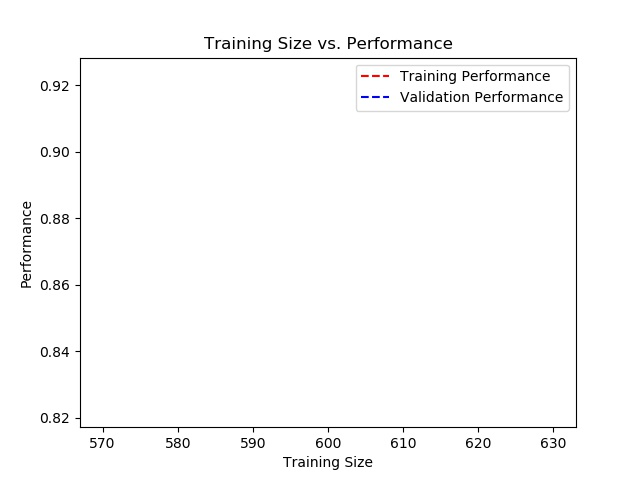
\includegraphics[scale=0.75, width=\linewidth]{Trainsize.jpg}
\caption{Graph comparing size of training set size vs. training accuracy and validation in increments of 50 images}
\label{fig:Trainsize}
\end{figure}
\end{center}
A potential explanation for the results in the figure may be that the training and validation sets, when split amongst the individual actors, may be favouring some actors over others.  There is an intersection at 100 training examples, and it appears the the accuracy between the two sets is almost identical.  The fact that there is a large discrepancy between the accuracies between a training sample size of ~180 to ~300 (e.g. validation accuracy stays relatively constant) may reveal support for the above claim that actors are not being represented properly, presumably due to a lack of rigour in the splitting between data sets for the individual actors.  Upon testing on the other actors and actresses not included in $act$, the validation accuracy obtained was $69\%$.  As outlined in the \textbf{Post-Mortem Addendum} in Section 2, the selection of data from the images may also have played a role in this behaviour.

\end{homeworkProblem}
\clearpage
%----------------------------------------------------------------------------------------
%----------------------------------------------------------------------------------------
%	PROBLEM 6
%----------------------------------------------------------------------------------------

\begin{homeworkProblem}
\noindent \textit{Mathematical Derivations of Gradient Descent}
\begin{enumerate}[label=(\Alph*)]
\item We can compute $\frac{\partial J}{\partial \theta_{pq}}$ by expanding the expression as outlined in the assignment documentation as follows:
\begin{center}
$J(\theta)=\sum_{i}\big((\theta^Tx^{(i)}-y^{(i)})^2_1+(\theta^Tx^{(i)}-y^{(i)})^2_2+\ldots+(\theta^Tx^{(i)}-y^{(i)})^1_j\big)$
\linebreak
$J(\theta)=(\theta^Tx^{(1)}-y^{(1)})^2_1+(\theta^Tx^{(1)}-y^{(1)})^2_2+\ldots(\theta^Tx^{(1)}-y^{(1)})^1_j+(\theta^Tx^{(2)}-y^{2)})^2_1+\ldots + (\theta^Tx^{(i)}-y^{(i)})^2_j$
\end{center}
Therefore, it appears we can model this double summation as a summation over the $p^{th}$ column and $q^{th}$ row.  Therefore, the partial derivative of a specific element, say, element $pq$ can be expressed as:
\begin{center}
$\boxed{\frac{\partial J}{\partial \theta _{pq}}=2x^{p}_{q}(\theta^T x^{p}-y^{p})_q}$
\end{center}
\item Based on the assignment specification, let $X$ be a matrix of size $n \times m$, where $n$ is the number of features and $m$ is the number of training examples.  Let $\theta$ be a matrix of size $k \times n$, where $k$ is the number of features.  Let $Y$ be a $k \times m$ matrix.  The provided expression taken from the assignment specification, with matrices substituted into their respective variables, gives the following expression:
\[2\begin{bmatrix}
x_{11} & \dots & x_{1m} \\
\vdots & \ddots & \vdots \\
x_{n1} & \dots & x_{nk}
\end{bmatrix}\times
\Bigg[\begin{bmatrix}
\theta_{11} & \dots & \theta_{1n} \\
\vdots & \ddots & \vdots \\
\theta_{k1} & \dots & \theta_{kn}
\end{bmatrix}^T \times
\begin{bmatrix}
x_{11} & \dots & x_{1m} \\
\vdots & \ddots & \vdots \\
x_{n1} & \dots & x_{nm}
\end{bmatrix} - 
\begin{bmatrix}
y_{11} & \dots & y_{1m} \\
\vdots & \ddots & \vdots \\
y_{k1} & \dots & y_{km}
\end{bmatrix}\Bigg]^T
\]

Simplification:
\[\begin{bmatrix}
2x_{11} & \dots & 2x_{1m} \\
\vdots & \ddots & \vdots \\
2x_{n1} & \dots & 2x_{nk}
\end{bmatrix}\times
\begin{bmatrix}
\theta_{11}x_{11}+\ldots +  \theta_{k1}x_{n1}-y_{11} & \dots \\
\vdots & \vdots  \\
\dots  & \theta_{1n}x_{1m}+\ldots+\theta_{kn}x_{nm}-y_{km}
\end{bmatrix}^T
\]
If the above matrix computation is carried out, we can observe, from part A, that the $pq$ term in the derivative of the cost function refers to an element within this gradient matrix.  For example, the top left hand side derivative, e.g. $\frac{\partial J}{\partial \theta_{11}}=2x_{11}(\theta_{11}x_{11}+\ldots + \theta_{k1}x_{n1}-y_{11}$.
\textbf{Note:}  The top left hand corner element of the gradient was selected for ease of computation, but any element within this gradient matrix would be valid.
\begin{lstlisting}
#Cost Function
def f2(x,y,theta):
    ones = np.ones((1,x.shape[1]))
    x = np.vstack((ones,x))
    hypothesis = np.matmul(theta.T,x)
    loss = np.power((hypothesis-y),2)
    return np.sum(loss)
\end{lstlisting}
\begin{lstlisting}
#Gradient Function
def df2(x,y,theta):
    ones = np.ones((1,x.shape[1]))
    x = vstack((ones,x))
    hypothesis = np.matmul(np.transpose(theta),x)-y
    hypothesis = np.transpose(hypothesis)
    gradient = 2*np.matmul(x,hypothesis)
    return gradient
\end{lstlisting}
\item The code for testing the implementation of the cost and gradient is shown below.
\begin{lstlisting}
#Testing the cost and gradient functionality
def part6():
    #Testing the loss function
    x = np.random.normal(0,0.6,(20,15))
    y = np.random.normal(0.2,0.4,(5,15))
    theta = np.random.normal(-0.1,0.3,(21,5))
    h = 0.00001
    #Cost of individual component
    testarr1 = np.zeros(theta.shape)
    testarr1[3,4] = h
    print("Cost is:")
    print((f2(x,y,theta+testarr1)-f2(x,y,theta-testarr1))/(2*h))
    print("Gradient is:")
    print(df2(x,y,theta)[3,4])
    testarr2 = np.zeros(theta.shape)
    testarr2[1,4] = h
    print("Cost is:")
    print((f2(x,y,theta+testarr2)-f2(x,y,theta-testarr2))/(2*h))
    print("Gradient is:")
    print(df2(x,y,theta)[1,4])
    testarr3 = np.zeros(theta.shape)
    testarr3[2,3] = h
    print("Cost is:")
    print((f2(x,y,theta+testarr3)-f2(x,y,theta-testarr3))/(2*h))
    print("Gradient is:")
    print(df2(x,y,theta)[2,3])
    testarr4 = np.zeros(theta.shape)
    testarr4[8,4] = h
    print("Cost is:")
    print((f2(x,y,theta+testarr4)-f2(x,y,theta-testarr4))/(2*h))
    print("Gradient is:")
    print(df2(x,y,theta)[8,4])
    testarr5 = np.zeros(theta.shape)
    testarr5[10,1] = h
    print("Cost is:")
    print((f2(x,y,theta+testarr5)-f2(x,y,theta-testarr5))/(2*h))
    print("Gradient is:")
    print(df2(x,y,theta)[10,1])
\end{lstlisting}
The output that results from execution of this code is below:
\begin{lstlisting}
Cost is:
-8.507892229658864
Gradient is:
-8.5078922306346
Cost is:
-5.070817460506305
Gradient is:
-5.070817460432679
Cost is:
-11.655092452400593
Gradient is:
-11.655092451975934
Cost is:
-3.5024079892309596
Gradient is:
-3.5024079896724483
Cost is:
-0.24353752436923057
Gradient is:
-0.2435375237734189
\end{lstlisting}
The $h$ was selected so as to try to compute a small difference, similar to the definition of the derivative - as $h$ further decreases, you would observe that the gradient and incremental difference in cost appear to converge.
\end{enumerate}

\end{homeworkProblem}
\clearpage
%----------------------------------------------------------------------------------------
%	PROBLEM 7
%----------------------------------------------------------------------------------------

\begin{homeworkProblem}

\noindent \textit{Linear Regression with Multiple Actors}

Running the linear regression classifier results in a training accuracy of $89\%$ and a validation accuracy of $56\%$.  Both the $\alpha$ and number of iterations were modified, to varying degrees of success - however, it is worth noting that the validation accuracy is significantly lower than the training accuracy which may be a symptom of overfitting.
\par Two loops were written in order to obtain the training hypothesis and validation hypothesis labels.  The steps are written below.
\begin{enumerate}
\item A matrix of 0's was initialized to the same shape as that of the label matrix
\item Each column in the label matrix was scanned for it's maximum value and the index of that value was stored in a new variable, \textit{max}
\item Starting at the $0^{th}$ column, a 1 was stored into the 0's matrix for each index in \textit{max}, and iterated through until the last column was reached.
\item The resultant matrix now had only one value of 1 in each column and was compared to the label matrix.
\end{enumerate}
An example of this for the training data is shown below.
\begin{lstlisting}
    #Training hypothesis
    ones_t = np.ones((1,training.shape[1]))
    training_with_bias = vstack((ones_t,training))
    training_hypothesis = np.matmul(theta.T,training_with_bias)
    max = training_hypothesis.argmax(axis=0)
    max = np.array(max)
    training_hypothesis_labels = np.zeros((training_hypothesis.shape))
    print(training_hypothesis_labels.shape)
    i = 0
    while i < training_hypothesis_labels.shape[1]:
        index = max[i]
        training_hypothesis_labels[index,i]=1
        i+=1

    correct = 0
    i = 0
    while i < training_hypothesis_labels.shape[1]:
        if np.array_equal(training_hypothesis_labels[:,i],training_labels[:,i]) is True:
            correct += 1
        i+=1
    print("Training accuracy is: " + str(correct/600.0))

\end{lstlisting}

\end{homeworkProblem}
\clearpage
%----------------------------------------------------------------------------------------
%	PROBLEM 8
%----------------------------------------------------------------------------------------
\begin{homeworkProblem}
\noindent \textit{Visualizing $\theta 's$ with multiple label matrix}

The 6 figures below show the visualized $\theta 's$ for training on the full set of actors in $act$ with the label matrix, as outlined in the assignment specification.
\begin{center}
\begin{figure}[!ht]\centering
\begin{subfigure}{.3\textwidth}\centering
  
\includegraphics[width=.3\linewidth]{thetas0.jpg}
  \caption{Baldwin $\theta 's$}
\end{subfigure}
\begin{subfigure}{.3\textwidth}\centering
  
\includegraphics[width=.3\linewidth]{thetas1.jpg}
  \caption{Bracco $\theta 's$}
\end{subfigure}
\begin{subfigure}{.3\textwidth}\centering
  
\includegraphics[width=.3\linewidth]{thetas2.jpg}
  \caption{Carell $\theta 's$}
\end{subfigure}
\begin{subfigure}{.3\textwidth}\centering
  
\includegraphics[width=.3\linewidth]{thetas3.jpg}
  \caption{Gilpin $\theta 's$}
\end{subfigure}
\begin{subfigure}{.3\textwidth}\centering
  
\includegraphics[width=.3\linewidth]{thetas4.jpg}
  \caption{Hader $\theta 's$}
\end{subfigure}
\begin{subfigure}{.3\textwidth}\centering
  
\includegraphics[width=.3\linewidth]{thetas5.jpg}
  \caption{Harmon $\theta 's$}
\end{subfigure}
\caption{$\theta$ values for each individual actor}
\end{figure}
\end{center}
A potential explanation for the lack of "face-like" appearance in $\theta 's $ obtained after training may be that the size of the training set is too large for each actor.  As observed in part 4, with only two actors from the Baldwin and Carell sets, the $\theta 's$ visualized more resembled faces.
\end{homeworkProblem}
\clearpage

%----------------------------------------------------------------------------------------
%	PROBLEM 8
%----------------------------------------------------------------------------------------
\begin{homeworkProblem}
\noindent \textit{Visualizing $\theta 's$ with multiple label matrix}

The 6 figures below show the visualized $\theta 's$ for training on the full set of actors in $act$ with the label matrix, as outlined in the assignment specification.
\begin{center}
\begin{figure}[!ht]\centering
\begin{subfigure}{.3\textwidth}\centering
  
\includegraphics[width=.3\linewidth]{thetas0.jpg}
  \caption{Baldwin $\theta 's$}
\end{subfigure}
\begin{subfigure}{.3\textwidth}\centering
  
\includegraphics[width=.3\linewidth]{thetas1.jpg}
  \caption{Bracco $\theta 's$}
\end{subfigure}
\begin{subfigure}{.3\textwidth}\centering
  
\includegraphics[width=.3\linewidth]{thetas2.jpg}
  \caption{Carell $\theta 's$}
\end{subfigure}
\begin{subfigure}{.3\textwidth}\centering
  
\includegraphics[width=.3\linewidth]{thetas3.jpg}
  \caption{Gilpin $\theta 's$}
\end{subfigure}
\begin{subfigure}{.3\textwidth}\centering
  
\includegraphics[width=.3\linewidth]{thetas4.jpg}
  \caption{Hader $\theta 's$}
\end{subfigure}
\begin{subfigure}{.3\textwidth}\centering
  
\includegraphics[width=.3\linewidth]{thetas5.jpg}
  \caption{Harmon $\theta 's$}
\end{subfigure}
\caption{$\theta$ values for each individual actor}
\end{figure}
\end{center}
A potential explanation for the lack of "face-like" appearance in $\theta 's $ obtained after training may be that the size of the training set is too large for each actor.  As observed in part 4, with only two actors from the Baldwin and Carell sets, the $\theta 's$ visualized more resembled faces.
\end{homeworkProblem}
\clearpage

%----------------------------------------------------------------------------------------
%	PROBLEM 8
%----------------------------------------------------------------------------------------
\begin{homeworkProblem}
\noindent \textit{Visualizing $\theta 's$ with multiple label matrix}

The 6 figures below show the visualized $\theta 's$ for training on the full set of actors in $act$ with the label matrix, as outlined in the assignment specification.
\begin{center}
\begin{figure}[!ht]\centering
\begin{subfigure}{.3\textwidth}\centering
  
\includegraphics[width=.3\linewidth]{thetas0.jpg}
  \caption{Baldwin $\theta 's$}
\end{subfigure}
\begin{subfigure}{.3\textwidth}\centering
  
\includegraphics[width=.3\linewidth]{thetas1.jpg}
  \caption{Bracco $\theta 's$}
\end{subfigure}
\begin{subfigure}{.3\textwidth}\centering
  
\includegraphics[width=.3\linewidth]{thetas2.jpg}
  \caption{Carell $\theta 's$}
\end{subfigure}
\begin{subfigure}{.3\textwidth}\centering
  
\includegraphics[width=.3\linewidth]{thetas3.jpg}
  \caption{Gilpin $\theta 's$}
\end{subfigure}
\begin{subfigure}{.3\textwidth}\centering
  
\includegraphics[width=.3\linewidth]{thetas4.jpg}
  \caption{Hader $\theta 's$}
\end{subfigure}
\begin{subfigure}{.3\textwidth}\centering
  
\includegraphics[width=.3\linewidth]{thetas5.jpg}
  \caption{Harmon $\theta 's$}
\end{subfigure}
\caption{$\theta$ values for each individual actor}
\end{figure}
\end{center}
A potential explanation for the lack of "face-like" appearance in $\theta 's $ obtained after training may be that the size of the training set is too large for each actor.  As observed in part 4, with only two actors from the Baldwin and Carell sets, the $\theta 's$ visualized more resembled faces.
\end{homeworkProblem}
\clearpage
\end{document}